% Brief: motivation (why anyone should care), principle of operation at a high level, what is new.
% Journalistic style: the first sentence of each paragraph says what it is about.

\begin{figure}[b]
  \centering
  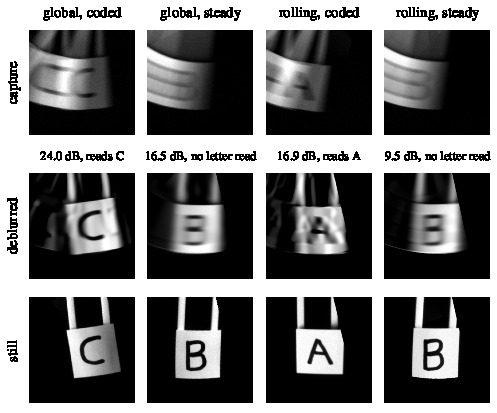
\includegraphics[width=\linewidth]{rig_cards}
  \caption{Coded light makes motion blur reversible, on the rig. The letter card on one blade of the fan
  turning at \SI{\rigCardSpeed}{rpm}, from the median capture (by PSNR) of each camera and light. Top: the
  capture, one exposure of 1.1 to \SI{1.4}{s}. Middle: our reconstruction, with its PSNR against the still
  and the letter a character reader finds in it. Bottom: a still of the stopped fan, turned onto the
  reconstructed blade. With coded light the letter comes back on both cameras, with some stripes left;
  with steady light of the same length it does not. Each panel is scaled to its own brightness.}
  \label{fig:rig-cards}
\end{figure}

 anything that moves forces a trade-off between blur and noise. A long exposure collects
enough light but smears the subject; a short one freezes it but is dark and noisy. Inspection of
rotating machinery, sport and traffic all suffer from this. Our test case is reading the letters on
the blades of a spinning fan, as one would read a marking on a rotating part without stopping it.

Ordinary motion blur cannot simply be undone. Under steady light a moving point traces a uniform
streak whose spectrum has exact zeros (\cref{fig:code}b), so detail at those frequencies is erased
and no algorithm can recover it. If the light is instead switched on and off in a well-chosen binary
code during the exposure, the blur keeps every frequency and becomes invertible~\cite{raskar2006coded}.

We build such a system with \emph{coded illumination}: a monitor beside the camera flashes the code
during one long exposure, so the camera needs no modification (\cref{fig:system}). The subject is a
fan with letters on its blades, driven by a stepper motor at a known speed. Unwrapping the image about
the hub turns the rotation into a shift, and the blur into a known linear operator that we invert
(\cref{fig:rig-cards}).

What is new is a three-way comparison of how the camera's shutter interacts with the code. A global
shutter exposes every row at once; a rolling shutter exposes row by row, so each row sees a different
part of the code. We reconstruct the rolling-shutter image with one blur for the whole frame or with
each row's own blur, and we also estimate the fan's speed from the photograph alone.

Our contributions are a coded illumination rig with a stepper-driven fan and both camera types
(\cref{sec:method}); an open reconstruction and speed estimation pipeline with automatic calibration;
and a measured comparison of coded against steady light on both cameras, with the three shutter
methods compared on the rig and in simulation, and a short exposure in simulation only
(\cref{sec:results}).
